\documentclass[conference]{IEEEtran}
\IEEEoverridecommandlockouts
% The preceding line is only needed to identify funding in the first footnote. If that is unneeded, please comment it out.
\usepackage{cite}
\usepackage{amsmath,amssymb,amsfonts}
\usepackage{algorithmic}
\usepackage{graphicx}
\usepackage{textcomp}
\usepackage{tabu}
\usepackage{multirow}
\usepackage{graphicx}
\usepackage{subfigure}
\usepackage{xcolor}
\usepackage[colorlinks,linkcolor=blue]{hyperref}
\usepackage{enumitem}
\newlist{subquestion}{enumerate}{1}
\setlist[subquestion,1]{label=(\alph*)}
\usepackage{listings}
\usepackage{pythonhighlight}
\usepackage{fancyhdr}
\pagestyle{fancy}
\cfoot{\thepage}


% flowchart
\usepackage{tikz,mathpazo}
\usetikzlibrary{shapes.geometric, arrows}
\usepackage{flowchart}

\def\BibTeX{{\rm B\kern-.05em{\sc i\kern-.025em b}\kern-.08em
    T\kern-.1667em\lower.7ex\hbox{E}\kern-.125emX}}

\setcounter{page}{1}
\begin{document}

\title{The Voice of Customers  \\
\begin{large} 
  CFPB data analysis from 2005 by now
\end{large} 
}

\author{\IEEEauthorblockN{Danfeng Wang}
\IEEEauthorblockA{\textit{Big Data Analytics} \\
\textit{Letterkeney Institute of Technology }\\
Donegal, Ireland \\
L00162010@student.lyit.ie }

}

\maketitle

\begin{abstract}
   This is a customer complaint dataset about the financial product consumption in the USA. We would like to hear the voice from these customers by analysing it. How many valid complaint data in this dataset? What is the most concerned problem? What is the strongest voice of these complaints? Have those financial companies improved their service from this? Can we predict the trends of the complaints?
   With these questions, we are going to have a exploration to this dataset. Please take a deep breath, hear the voices from the customers. Let the millions of complaints records tell us the truth, charts never lie.
\end{abstract}


\section{Introduction}

The dataset of this project obtained from the data.gov website is a database of consumers’ complaints about financial products collected by the Consumer Financial Protection Bureau, an agency of the United States government responsible for consumer protection in the financial sector USA \cite{datasource}.

The analysis of this dataset can be used for  finding common problems of products in financial sector and making precautions. By using data visualization and machine learning approach, this report gives insights and understanding into consumers perspective so that to provide ideas of how to improve control measures in financial products or give better regulations and decisions in the management of the financial market.
\begin{itemize}
\item What's the most complained from different dimensions, such as complained channels,companies, products. Have they changed over time?

\item Pictures speak louder than text, what can we get from the narrative of those complaints.

\item Can we predict the issue type? Can we predict the process result to guide the urgency of these complaints, so that the companies can give a  higher priority when dealing with the urgent complaints.
\item The quality of service - responding time, where, what and which providers got the most complaints. Any improvement later? 

\end{itemize}

\section{Code list}

\section{System preparation}\label{AA}
We apply big data and machine learning related techniques to implement this project. The goal of the project as follows:
\begin{enumerate}[label=(\roman*)]
\item providing descriptive analysis combined with visualization, such as bar charts and word cloud charts
\item providing prediction model by training the dataset
\end{enumerate}

In the process of achieving the above goal, we have three aspects to consider:

\textbf{Data engineering
}\begin{itemize}
\item  - data ingestion
\item - data preparation 
\item - visualization
\end{itemize}


\textbf{Machine learning
}\begin{itemize}
\item  - data loading
\item - feature engineering
\item - training and prediction
\item - model tuning 
\end{itemize}







Databrick is a cloud platform for big data analysis. In this project, we use Databrick as the data storage, analysis and modelling platform.
Follow the next steps for system preparation.
\begin{itemize}

\item Sign up for a free Databrick trial.
\item Create a cluster 6.4 (includes Apache Spark 2.4.5, Scala 2.11) 
\item Create notebook.
\item Start cluster.
The cluster will be terminated automatically after 60 minutes of inactivity.
\end{itemize}

At the data modelling stage, we use MLFlow on Databrick to implement the machine learning pipeline. MLFlow is an platform for managing the machine learning lifecycle.  


\section{Dataset acquisition}

The volume of this dataset is roughly 2 million items. It includes complaints dating from 2015 to the end of 2017. 

\begin{itemize}
\item Download dataset file from the web site.
\item Upload the file into DBFS. 
\item Unzip and load the data into table.
\item Check the integrity.
\end{itemize}
During this process, we found the csv format cannot be correctly loaded by spark SQLContext, . By reading few line from the file, we found the fields are seperated by comma, one of the descriptive field \emph{Consumer complaint narrative} is enclosed by double quotes. By applying loading parameters such as \emph{escape} and \emph{quotion}, the problem remained.
In order to avoid this problem, we tried loading json file.

\subsection{Fields description}\label{AA}
see Table1.
\begin{itemize}
\item \textit{Company public response} - standard items. This is how the company attributed the complaint. Some are believed the company should not be responsible for the issue, it should be a third party, policy, consumer, misunderstanding and so forth. Some are resolved privately which we can not distinguish the attribute, and some are believed invalid complaints.
\item \textit{Company response to consumer} - The process status is close, in progress or untimely response in which the close status has several different way including close with explanation, monetary relief, non-monetary relief, relief or without relief. We can see percentage of issue resolved and in which way the issues have been resolved.  
\item \textit{Product} - Does the products complained distributed evenly? Which products are the most complained? Are the products complained by consumers changed within these years, and whether the changes are influenced by the complaints data..
\end{itemize}

\begin{table}[h]
\caption{Dataset Structure}
\begin{tabular}{p{1cm}|p{1.5cm}|p{0.7cm}|p{3.5cm}}
\hline
\hline
Category & Field & Format & Remark \\ \hline
identity & Complaint ID & integer & identity of a complaint record  
\\ \hline
data source & Submitted via & dict & Email,Fax,Phone,Postal mail,Referral,Web  
\\ \hline
\multirow{2}{*}{date} & Date Received & yyyy-mm-dd & received date  
\\ \cline{2-4}
 & Date sent to company & yyyy-mm-dd & Date sent to company  
\\ \hline
\multirow{5}{*}{company} & Company public response & string & Company public response  \\ \cline{2-4}
 & Company  & string & Company name \\ \cline{2-4}
 & Company response to consumer  & dict/null & Company response to consumer \\ \cline{2-4}
 & Consumer consent provided?  & Yes/No & Consumer consent provided \\ \cline{2-4}
 & Timely response?  & Yes/No & Timely response? \\ \hline
\multirow{2}{*}{product} & Product  & string & \\ \cline{2-4}
 & Sub-product  & string & \\ \hline
\multirow{6}{*}{issue} & Issue  & string & \\ \cline{2-4}
 & Sub-issue  & string & \\ \cline{2-4}
 & Consumer complaint narrative  & string & \\ \cline{2-4}
 & Consumer disputed?  & Yes/No & \\ \cline{2-4}
 & State  & dict & \\ \cline{2-4}
 & ZIP code  & dict & \\ \hline
\hline
\end{tabular}
\end{table}

\subsection{Target fields}\label{AA}
By reading this dataset, we can categorize the columns of the dataset into the following:
\begin{itemize}
\item date: received date and sent date.
\item location: ZIP code, State and so forth.
\item standardized text:
\item narrative text: 
\item state related fields: Yes/No states.
\end{itemize}

\subsection{Business process}\label{AA}
The complaint data will go through the following steps when it is submitted to the CFPB.

 % basic shape of the flowchart
\tikzstyle{startstop} = [rectangle, rounded corners, minimum width=3cm, minimum height=1cm,text centered, draw=black, fill=red!30]
\tikzstyle{io} = [trapezium, trapezium left angle=70, trapezium right angle=110, minimum width=3cm, minimum height=1cm, text centered, draw=black, fill=blue!30]
\tikzstyle{process} = [rectangle, minimum width=3cm, minimum height=1cm, text centered, draw=black, fill=orange!30]
\tikzstyle{decision} = [diamond, minimum width=3cm, minimum height=1cm, text centered, draw=black, fill=green!30]
\tikzstyle{arrow} = [thick,->,>=stealth]

\begin{tikzpicture}[node distance=1.5cm]
\node (start) [startstop] {Complaint submitted};
\node (in1) [io, below of=start] {Review and route};
\node (pro1) [process, below of=in1] {Company response};
\node (pro2) [process, below of=pro1, yshift=-0.5cm] {Complaint published};
\node (stop) [startstop, below of=pro2] {Consumer review};

\draw [arrow](start) -- (in1);
\draw [arrow](in1) -- (pro1);
\draw [arrow](pro1) -- (pro2);
\draw [arrow](pro2) -- (stop);
\end{tikzpicture}

\subsection{More about the data}\label{AA}
The complaint facts will not be verified by CFPB, but it gives the companies opportunity to confirm the consumer has commercial relationship with them. 



\section{Data preparation}\label{AA}
In order to make it easier to manipulate in the next stages, the dataset will be prepared as follows:

\subsection{Data integration}\label{AA}
The purpose of this stage is to make sure the dataset is analysable.

By looking at the data, 
\begin{itemize}
\item check null value to target fields.
\item validate the date fields.
\item Check the value of state fields.Standardizing?
\\item type conversion.
\\item eliminating meaningless words such as stop words, symbols, and convert the text into lower case.
\end{itemize}



\subsection{Data transformation}\label{AA}
\begin{itemize}

\item date: generate corresponding fields such as year, month, week and so forth.
\item location: generate geographical columns, such as longitude, latitude and so forth.
\item standardized text: convert text to code. Split the text into words, extract nouns.
\end{itemize}


\section{Data aggregation}\label{AA}

\section{Data analysis}\label{AA}
\subsection{What products they are complaining about}\label{AA}


\section{Method}

\subsection{Tools and architecture }\label{AA}
Figure x shows the workflow of this research including data source, method and data analysis.
Data pre-processing: clean noise data.

After pre-processing, sentiment analysis will be applied on this dataset.


\subsection{Data modelling }\label{AA}
This is a time series based dataset

\section{Related work}

The initial goal focuses on the following points:

\subsection{Descriptive Analysis}\label{AA}

\begin{itemize}

\item The composition of these complaints by multiple dimensions.

From multiple aspects to give an insight of this dataset, such as company, product, issue, submitted channel. By using annually grouped bar chart, we can see the proportion of each kind of these most complaints from different perspective.

\item The complaints reason rank.
\item Time series analysis, such as year-on-year, month-on-month comparison.
\item Complains distribution by multiple dimension.
\item In-depth analysis if any outlier is found in the above.
\end{itemize}


\subsection{Predictive Analysis}

\begin{itemize}

\item Complaint trends prediction.
\item Identify the problems within the complaints which tends to cause more complaints.
\end{itemize}


\subsection{Sentiment Analysis}

\begin{itemize}

\item Word cloud : This is a visualization form for representing large amount of text by using different font size and color to give the most frequently appeared words visual prominence.
\item Identify the problems within the complaints which tends to cause more complaints.
\end{itemize}

\section{Descriptive analysis }

\begin{itemize}
\item Show the rank of total number of complaints based on different dimensions. 
In this process, we visualized the data from different dimensions to see how many complaints happened, as well as the trend over time.

For example, the figure x shows the top 4 complained companies. 
From annually top 4 ranked complaints  by product, we can see
during the first 4 years of the survey period, the amount of complaints are focus on mortgage and continues to decline after 2013. The complaints of credit reporting product appeared in 2017 and showed rapid growth in recent years.
- the top N ranked states chart shows that the amount of complaints in the state is proportional to that of the population.


	\begin{figure}[h]
		\centering
		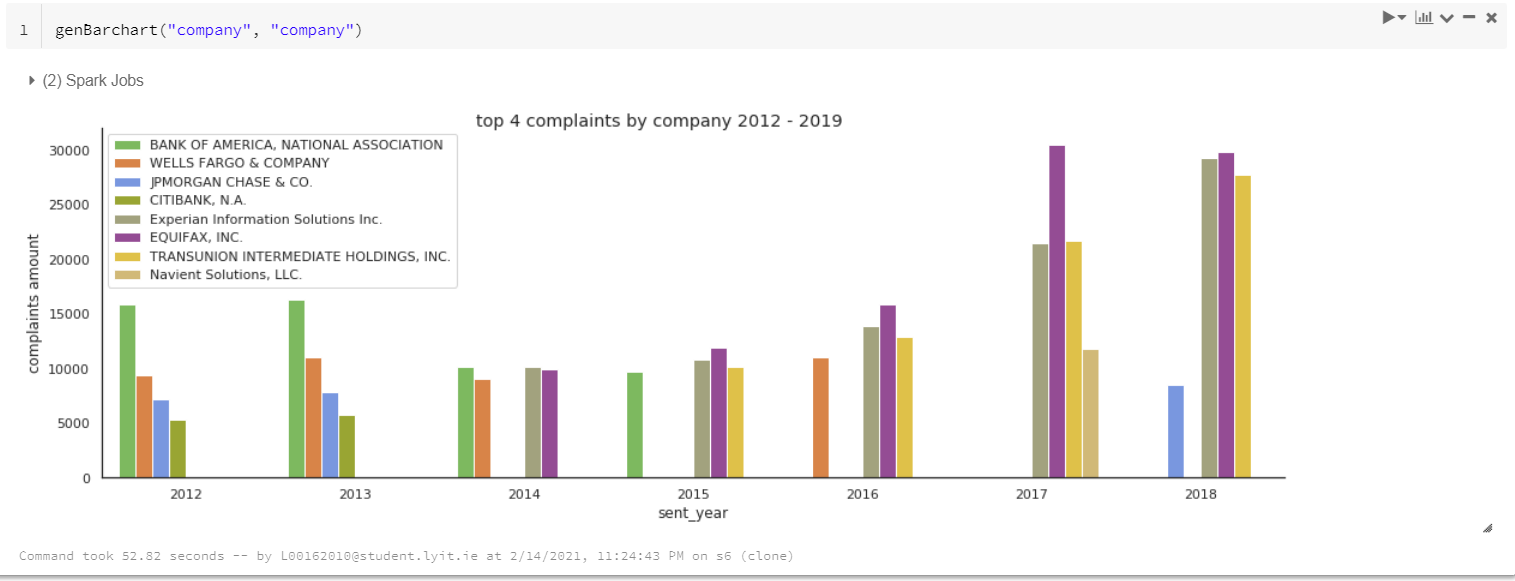
\includegraphics[width=1\linewidth]{img/bycompany.png}
	\end{figure} 






\item Word cloud - the consumers' complaints cannot be described clearly by only categories or single words, so what happened is collected through narrative text in this dataset. This will be helpful for exploring the descriptive text. In this project, we process the narrative text by the following steps.

\begin{enumerate}
\item normalization - convert the text content into lower case and remove the non words such as punctuation.
\item tokenization - split the sentences into words.
\item stop words -  
\item tagging - only keep specific word types, such as noun.
\item stemming - reducing the words to it's word stem so that the similar words lie under a same stem.
\end{enumerate}

After the above process, we calculated the numbers of these words and visualize it  by wordscloud chart. The below images shows the wordscloud chart based on the product of Student Load

	\begin{figure}[h]
		\centering
		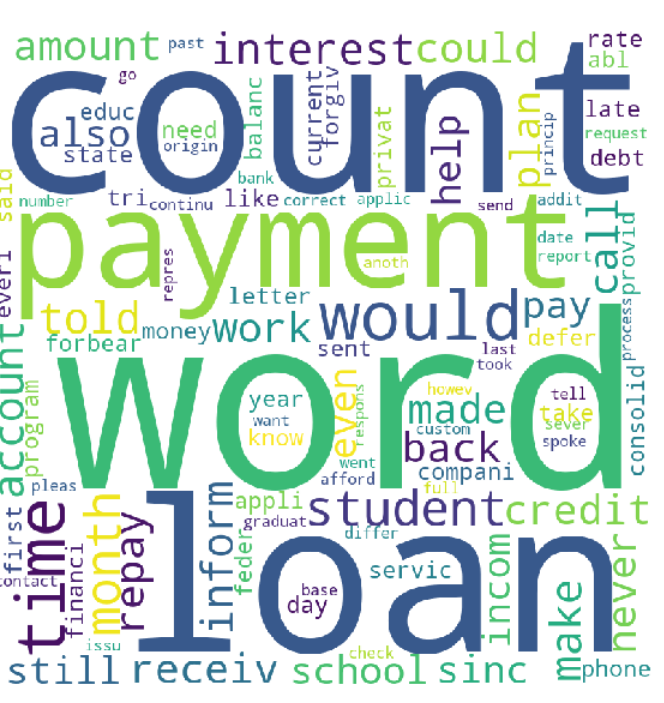
\includegraphics[width=.8\linewidth]{img/word_cloud_student.png}
	\end{figure} 

\end{itemize}

\section{Predictive analysis }
When exploring this dataset, we found the part of within company response column, there are several ways for the company to deal with the issues. Some of the response involved with money or other non-monetary relief. It would be a valuable reference for the companies complained by the customers if we are able to predict the settlement whether involves with any forms of relief or not? 

\section{Conclusion }

From the above analysis, we have heard the voices from the customers in consuming financial products. From this process of manipulating this dataset, we have known the pipeline of dealing with big data. Big data is able to offer us insights into what happened in the financial products domain as well as the prediction of what will happen. 
For further analysis, we plan to continue to providing more visualizations combined with multi dimensions, for example, analysis the data base on geographical features. Moreover, the nlp sentiment analysis.   
 
\textbf{Feature selection} - to evaluate which features we will use to train the model.

\textbf{Cross-validation} - we prepare the dataset by using 5-folder cross-validation. This is a popular method which tends to provide less biased model than a simple $train_test_split$.

\textbf{model selection} - 

\textbf{model tuning} - 


\begin{itemize}
\item feature selection
\item one-hot encoding (Bag of words) - It represent the sentence by replacing each unique word into a specific number. With this Bag of Words model, the sequence of the words is ignored.
\item relevant - plot the information. Since we have many categorical features in the dataset, we  apply PCA to do dimensionality deduction. 
\item classification - Logistic Regression, which is simple and explainable. 
\end{itemize}

\section{Future work}

The analysis will be done by using Python notebook on Google Colab. The process of the analysis is listed as follows:

\begin{itemize}
\item data understanding - get domain knowledge by doing research according to the data.
\item Data preparation – download and unzip data from data.gov . Check data integrity and outliers, process Null cells, unuseful rows or columns which have less relevant with the main purpose of this analytical work.Data type and calculated fields process and so forth.
\item Data visualization – Implement the descriptive analysis.
\item Data prediction – data modeling with multiple algorithms and optimization and evaluation of the models. The complaints prediction is a classification problem.
\begin{enumerate}
\item training - split the dataset for training and testing. 
\item apply Logistic Regression to train and predict. 
\item Try to understandand the error rate of the model, reference from \href{https://www.kdnuggets.com/2019/01/solve-90-nlp-problems-step-by-step-guide.html}{nlp} \begin{quotation} A first step is to understand the types of errors our model makes, and which kind of errors are least desirable. In our example, false positives are classifying an irrelevant tweet as a disaster, and false negatives are classifying a disaster as an irrelevant tweet. If the priority is to react to every potential event, we would want to lower our false negatives. If we are constrained in resources however, we might prioritize a lower false positive rate to reduce false alarms. A good way to visualize this information is using a Confusion Matrix, which compares the predictions our model makes with the true label. Ideally, the matrix would be a diagonal line from top left to bottom right (our predictions match the truth perfectly)."\end{quotation}

\end{enumerate}

\end{itemize}

\begin{thebibliography}{9}
\bibitem{datasource} 
https://catalog.data.gov/dataset/consumer-complaint-database. 
\textit{The \LaTeX\ Companion}. 
The Consumer Complaint Database, Metadata Updated: July 17, 2020.

\bibitem{fields} 
https://cfpb.github.io/api/ccdb/fields.html
\textit{The \LaTeX\ Companion}. 
The Consumer Complaint Database fields description.

\bibitem{fields_changes} 
(“Summary of product and sub-product changes,” n.d.) 

\end{thebibliography}
\end{document}
